% Created by tikzDevice version 0.10.1 on 2017-10-30 17:28:49
% !TEX encoding = UTF-8 Unicode
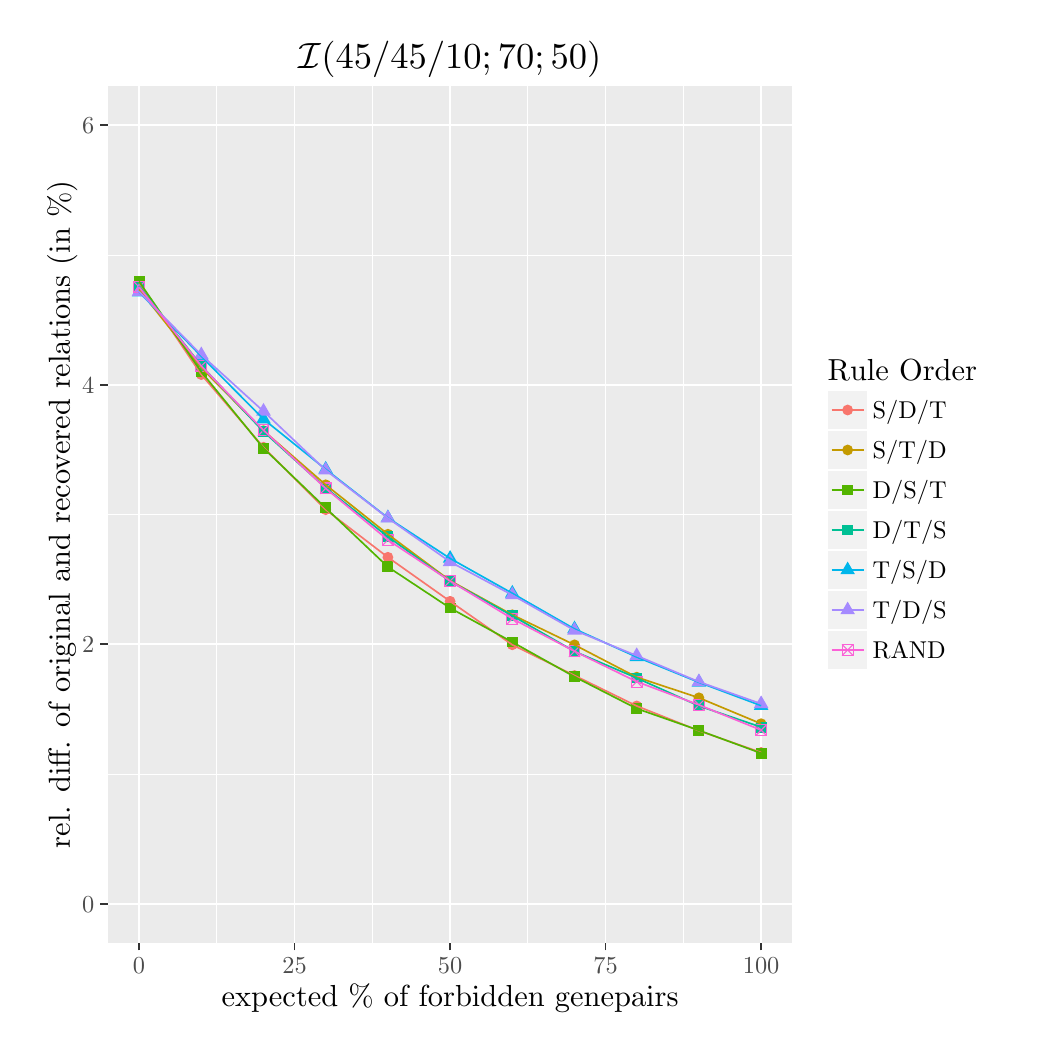
\begin{tikzpicture}[x=1pt,y=1pt]
\definecolor{fillColor}{RGB}{255,255,255}
\path[use as bounding box,fill=fillColor,fill opacity=0.00] (0,0) rectangle (361.35,361.35);
\begin{scope}
\path[clip] (  0.00,  0.00) rectangle (361.35,361.35);
\definecolor{drawColor}{RGB}{255,255,255}
\definecolor{fillColor}{RGB}{255,255,255}

\path[draw=drawColor,line width= 0.6pt,line join=round,line cap=round,fill=fillColor] (  0.00,  0.00) rectangle (361.35,361.35);
\end{scope}
\begin{scope}
\path[clip] ( 29.02, 30.69) rectangle (276.26,340.16);
\definecolor{fillColor}{gray}{0.92}

\path[fill=fillColor] ( 29.02, 30.69) rectangle (276.26,340.16);
\definecolor{drawColor}{RGB}{255,255,255}

\path[draw=drawColor,line width= 0.3pt,line join=round] ( 29.02, 91.64) --
	(276.26, 91.64);

\path[draw=drawColor,line width= 0.3pt,line join=round] ( 29.02,185.42) --
	(276.26,185.42);

\path[draw=drawColor,line width= 0.3pt,line join=round] ( 29.02,279.20) --
	(276.26,279.20);

\path[draw=drawColor,line width= 0.3pt,line join=round] ( 68.36, 30.69) --
	( 68.36,340.16);

\path[draw=drawColor,line width= 0.3pt,line join=round] (124.55, 30.69) --
	(124.55,340.16);

\path[draw=drawColor,line width= 0.3pt,line join=round] (180.74, 30.69) --
	(180.74,340.16);

\path[draw=drawColor,line width= 0.3pt,line join=round] (236.93, 30.69) --
	(236.93,340.16);

\path[draw=drawColor,line width= 0.6pt,line join=round] ( 29.02, 44.75) --
	(276.26, 44.75);

\path[draw=drawColor,line width= 0.6pt,line join=round] ( 29.02,138.53) --
	(276.26,138.53);

\path[draw=drawColor,line width= 0.6pt,line join=round] ( 29.02,232.31) --
	(276.26,232.31);

\path[draw=drawColor,line width= 0.6pt,line join=round] ( 29.02,326.09) --
	(276.26,326.09);

\path[draw=drawColor,line width= 0.6pt,line join=round] ( 40.26, 30.69) --
	( 40.26,340.16);

\path[draw=drawColor,line width= 0.6pt,line join=round] ( 96.45, 30.69) --
	( 96.45,340.16);

\path[draw=drawColor,line width= 0.6pt,line join=round] (152.64, 30.69) --
	(152.64,340.16);

\path[draw=drawColor,line width= 0.6pt,line join=round] (208.83, 30.69) --
	(208.83,340.16);

\path[draw=drawColor,line width= 0.6pt,line join=round] (265.03, 30.69) --
	(265.03,340.16);
\definecolor{fillColor}{RGB}{248,118,109}

\path[fill=fillColor] ( 40.26,269.37) circle (  1.96);

\path[fill=fillColor] ( 62.74,235.99) circle (  1.96);

\path[fill=fillColor] ( 85.22,209.73) circle (  1.96);

\path[fill=fillColor] (107.69,187.18) circle (  1.96);

\path[fill=fillColor] (130.17,169.97) circle (  1.96);

\path[fill=fillColor] (152.64,154.07) circle (  1.96);

\path[fill=fillColor] (175.12,138.36) circle (  1.96);

\path[fill=fillColor] (197.60,127.25) circle (  1.96);

\path[fill=fillColor] (220.07,116.25) circle (  1.96);

\path[fill=fillColor] (242.55,107.30) circle (  1.96);

\path[fill=fillColor] (265.03, 99.43) circle (  1.96);
\definecolor{fillColor}{RGB}{196,154,0}

\path[fill=fillColor] ( 40.26,266.73) circle (  1.96);

\path[fill=fillColor] ( 62.74,238.45) circle (  1.96);

\path[fill=fillColor] ( 85.22,215.72) circle (  1.96);

\path[fill=fillColor] (107.69,196.16) circle (  1.96);

\path[fill=fillColor] (130.17,178.30) circle (  1.96);

\path[fill=fillColor] (152.64,161.54) circle (  1.96);

\path[fill=fillColor] (175.12,149.18) circle (  1.96);

\path[fill=fillColor] (197.60,138.33) circle (  1.96);

\path[fill=fillColor] (220.07,126.65) circle (  1.96);

\path[fill=fillColor] (242.55,119.20) circle (  1.96);

\path[fill=fillColor] (265.03,109.83) circle (  1.96);
\definecolor{fillColor}{RGB}{83,180,0}

\path[fill=fillColor] ( 38.30,267.62) --
	( 42.23,267.62) --
	( 42.23,271.55) --
	( 38.30,271.55) --
	cycle;

\path[fill=fillColor] ( 60.78,235.03) --
	( 64.70,235.03) --
	( 64.70,238.96) --
	( 60.78,238.96) --
	cycle;

\path[fill=fillColor] ( 83.25,207.41) --
	( 87.18,207.41) --
	( 87.18,211.34) --
	( 83.25,211.34) --
	cycle;

\path[fill=fillColor] (105.73,185.85) --
	(109.65,185.85) --
	(109.65,189.77) --
	(105.73,189.77) --
	cycle;

\path[fill=fillColor] (128.21,164.53) --
	(132.13,164.53) --
	(132.13,168.46) --
	(128.21,168.46) --
	cycle;

\path[fill=fillColor] (150.68,149.68) --
	(154.61,149.68) --
	(154.61,153.61) --
	(150.68,153.61) --
	cycle;

\path[fill=fillColor] (173.16,137.38) --
	(177.08,137.38) --
	(177.08,141.31) --
	(173.16,141.31) --
	cycle;

\path[fill=fillColor] (195.63,124.83) --
	(199.56,124.83) --
	(199.56,128.75) --
	(195.63,128.75) --
	cycle;

\path[fill=fillColor] (218.11,113.33) --
	(222.04,113.33) --
	(222.04,117.26) --
	(218.11,117.26) --
	cycle;

\path[fill=fillColor] (240.59,105.48) --
	(244.51,105.48) --
	(244.51,109.40) --
	(240.59,109.40) --
	cycle;

\path[fill=fillColor] (263.06, 97.20) --
	(266.99, 97.20) --
	(266.99,101.13) --
	(263.06,101.13) --
	cycle;
\definecolor{fillColor}{RGB}{0,192,148}

\path[fill=fillColor] ( 38.30,266.03) --
	( 42.23,266.03) --
	( 42.23,269.95) --
	( 38.30,269.95) --
	cycle;

\path[fill=fillColor] ( 60.78,237.24) --
	( 64.70,237.24) --
	( 64.70,241.16) --
	( 60.78,241.16) --
	cycle;

\path[fill=fillColor] ( 83.25,213.43) --
	( 87.18,213.43) --
	( 87.18,217.36) --
	( 83.25,217.36) --
	cycle;

\path[fill=fillColor] (105.73,193.10) --
	(109.65,193.10) --
	(109.65,197.03) --
	(105.73,197.03) --
	cycle;

\path[fill=fillColor] (128.21,175.43) --
	(132.13,175.43) --
	(132.13,179.36) --
	(128.21,179.36) --
	cycle;

\path[fill=fillColor] (150.68,159.35) --
	(154.61,159.35) --
	(154.61,163.27) --
	(150.68,163.27) --
	cycle;

\path[fill=fillColor] (173.16,146.88) --
	(177.08,146.88) --
	(177.08,150.81) --
	(173.16,150.81) --
	cycle;

\path[fill=fillColor] (195.63,134.00) --
	(199.56,134.00) --
	(199.56,137.92) --
	(195.63,137.92) --
	cycle;

\path[fill=fillColor] (218.11,124.38) --
	(222.04,124.38) --
	(222.04,128.30) --
	(218.11,128.30) --
	cycle;

\path[fill=fillColor] (240.59,114.31) --
	(244.51,114.31) --
	(244.51,118.23) --
	(240.59,118.23) --
	cycle;

\path[fill=fillColor] (263.06,106.65) --
	(266.99,106.65) --
	(266.99,110.57) --
	(263.06,110.57) --
	cycle;
\definecolor{fillColor}{RGB}{0,182,235}

\path[fill=fillColor] ( 40.26,268.86) --
	( 42.91,264.28) --
	( 37.62,264.28) --
	cycle;

\path[fill=fillColor] ( 62.74,245.65) --
	( 65.38,241.07) --
	( 60.10,241.07) --
	cycle;

\path[fill=fillColor] ( 85.22,222.93) --
	( 87.86,218.35) --
	( 82.57,218.35) --
	cycle;

\path[fill=fillColor] (107.69,204.82) --
	(110.33,200.24) --
	(105.05,200.24) --
	cycle;

\path[fill=fillColor] (130.17,187.27) --
	(132.81,182.69) --
	(127.53,182.69) --
	cycle;

\path[fill=fillColor] (152.64,172.61) --
	(155.29,168.03) --
	(150.00,168.03) --
	cycle;

\path[fill=fillColor] (175.12,160.01) --
	(177.76,155.44) --
	(172.48,155.44) --
	cycle;

\path[fill=fillColor] (197.60,147.13) --
	(200.24,142.55) --
	(194.95,142.55) --
	cycle;

\path[fill=fillColor] (220.07,136.98) --
	(222.72,132.41) --
	(217.43,132.41) --
	cycle;

\path[fill=fillColor] (242.55,127.84) --
	(245.19,123.26) --
	(239.91,123.26) --
	cycle;

\path[fill=fillColor] (265.03,119.41) --
	(267.67,114.83) --
	(262.38,114.83) --
	cycle;
\definecolor{fillColor}{RGB}{165,138,255}

\path[fill=fillColor] ( 40.26,268.99) --
	( 42.91,264.41) --
	( 37.62,264.41) --
	cycle;

\path[fill=fillColor] ( 62.74,246.16) --
	( 65.38,241.58) --
	( 60.10,241.58) --
	cycle;

\path[fill=fillColor] ( 85.22,225.77) --
	( 87.86,221.19) --
	( 82.57,221.19) --
	cycle;

\path[fill=fillColor] (107.69,204.50) --
	(110.33,199.92) --
	(105.05,199.92) --
	cycle;

\path[fill=fillColor] (130.17,187.17) --
	(132.81,182.59) --
	(127.53,182.59) --
	cycle;

\path[fill=fillColor] (152.64,171.40) --
	(155.29,166.82) --
	(150.00,166.82) --
	cycle;

\path[fill=fillColor] (175.12,159.38) --
	(177.76,154.81) --
	(172.48,154.81) --
	cycle;

\path[fill=fillColor] (197.60,146.64) --
	(200.24,142.06) --
	(194.95,142.06) --
	cycle;

\path[fill=fillColor] (220.07,137.46) --
	(222.72,132.88) --
	(217.43,132.88) --
	cycle;

\path[fill=fillColor] (242.55,128.03) --
	(245.19,123.45) --
	(239.91,123.45) --
	cycle;

\path[fill=fillColor] (265.03,120.08) --
	(267.67,115.51) --
	(262.38,115.51) --
	cycle;
\definecolor{drawColor}{RGB}{251,97,215}

\path[draw=drawColor,line width= 0.4pt,line join=round,line cap=round] ( 38.30,265.68) rectangle ( 42.23,269.60);

\path[draw=drawColor,line width= 0.4pt,line join=round,line cap=round] ( 38.30,265.68) -- ( 42.23,269.60);

\path[draw=drawColor,line width= 0.4pt,line join=round,line cap=round] ( 38.30,269.60) -- ( 42.23,265.68);

\path[draw=drawColor,line width= 0.4pt,line join=round,line cap=round] ( 60.78,237.13) rectangle ( 64.70,241.05);

\path[draw=drawColor,line width= 0.4pt,line join=round,line cap=round] ( 60.78,237.13) -- ( 64.70,241.05);

\path[draw=drawColor,line width= 0.4pt,line join=round,line cap=round] ( 60.78,241.05) -- ( 64.70,237.13);

\path[draw=drawColor,line width= 0.4pt,line join=round,line cap=round] ( 83.25,213.92) rectangle ( 87.18,217.85);

\path[draw=drawColor,line width= 0.4pt,line join=round,line cap=round] ( 83.25,213.92) -- ( 87.18,217.85);

\path[draw=drawColor,line width= 0.4pt,line join=round,line cap=round] ( 83.25,217.85) -- ( 87.18,213.92);

\path[draw=drawColor,line width= 0.4pt,line join=round,line cap=round] (105.73,192.90) rectangle (109.65,196.82);

\path[draw=drawColor,line width= 0.4pt,line join=round,line cap=round] (105.73,192.90) -- (109.65,196.82);

\path[draw=drawColor,line width= 0.4pt,line join=round,line cap=round] (105.73,196.82) -- (109.65,192.90);

\path[draw=drawColor,line width= 0.4pt,line join=round,line cap=round] (128.21,174.29) rectangle (132.13,178.21);

\path[draw=drawColor,line width= 0.4pt,line join=round,line cap=round] (128.21,174.29) -- (132.13,178.21);

\path[draw=drawColor,line width= 0.4pt,line join=round,line cap=round] (128.21,178.21) -- (132.13,174.29);

\path[draw=drawColor,line width= 0.4pt,line join=round,line cap=round] (150.68,159.44) rectangle (154.61,163.37);

\path[draw=drawColor,line width= 0.4pt,line join=round,line cap=round] (150.68,159.44) -- (154.61,163.37);

\path[draw=drawColor,line width= 0.4pt,line join=round,line cap=round] (150.68,163.37) -- (154.61,159.44);

\path[draw=drawColor,line width= 0.4pt,line join=round,line cap=round] (173.16,145.81) rectangle (177.08,149.74);

\path[draw=drawColor,line width= 0.4pt,line join=round,line cap=round] (173.16,145.81) -- (177.08,149.74);

\path[draw=drawColor,line width= 0.4pt,line join=round,line cap=round] (173.16,149.74) -- (177.08,145.81);

\path[draw=drawColor,line width= 0.4pt,line join=round,line cap=round] (195.63,134.04) rectangle (199.56,137.96);

\path[draw=drawColor,line width= 0.4pt,line join=round,line cap=round] (195.63,134.04) -- (199.56,137.96);

\path[draw=drawColor,line width= 0.4pt,line join=round,line cap=round] (195.63,137.96) -- (199.56,134.04);

\path[draw=drawColor,line width= 0.4pt,line join=round,line cap=round] (218.11,123.07) rectangle (222.04,126.99);

\path[draw=drawColor,line width= 0.4pt,line join=round,line cap=round] (218.11,123.07) -- (222.04,126.99);

\path[draw=drawColor,line width= 0.4pt,line join=round,line cap=round] (218.11,126.99) -- (222.04,123.07);

\path[draw=drawColor,line width= 0.4pt,line join=round,line cap=round] (240.59,114.67) rectangle (244.51,118.59);

\path[draw=drawColor,line width= 0.4pt,line join=round,line cap=round] (240.59,114.67) -- (244.51,118.59);

\path[draw=drawColor,line width= 0.4pt,line join=round,line cap=round] (240.59,118.59) -- (244.51,114.67);

\path[draw=drawColor,line width= 0.4pt,line join=round,line cap=round] (263.06,105.56) rectangle (266.99,109.48);

\path[draw=drawColor,line width= 0.4pt,line join=round,line cap=round] (263.06,105.56) -- (266.99,109.48);

\path[draw=drawColor,line width= 0.4pt,line join=round,line cap=round] (263.06,109.48) -- (266.99,105.56);
\definecolor{drawColor}{RGB}{248,118,109}

\path[draw=drawColor,line width= 0.6pt,line join=round] ( 40.26,269.37) --
	( 62.74,235.99) --
	( 85.22,209.73) --
	(107.69,187.18) --
	(130.17,169.97) --
	(152.64,154.07) --
	(175.12,138.36) --
	(197.60,127.25) --
	(220.07,116.25) --
	(242.55,107.30) --
	(265.03, 99.43);
\definecolor{drawColor}{RGB}{196,154,0}

\path[draw=drawColor,line width= 0.6pt,line join=round] ( 40.26,266.73) --
	( 62.74,238.45) --
	( 85.22,215.72) --
	(107.69,196.16) --
	(130.17,178.30) --
	(152.64,161.54) --
	(175.12,149.18) --
	(197.60,138.33) --
	(220.07,126.65) --
	(242.55,119.20) --
	(265.03,109.83);
\definecolor{drawColor}{RGB}{83,180,0}

\path[draw=drawColor,line width= 0.6pt,line join=round] ( 40.26,269.59) --
	( 62.74,236.99) --
	( 85.22,209.37) --
	(107.69,187.81) --
	(130.17,166.49) --
	(152.64,151.64) --
	(175.12,139.34) --
	(197.60,126.79) --
	(220.07,115.30) --
	(242.55,107.44) --
	(265.03, 99.16);
\definecolor{drawColor}{RGB}{0,192,148}

\path[draw=drawColor,line width= 0.6pt,line join=round] ( 40.26,267.99) --
	( 62.74,239.20) --
	( 85.22,215.39) --
	(107.69,195.06) --
	(130.17,177.40) --
	(152.64,161.31) --
	(175.12,148.85) --
	(197.60,135.96) --
	(220.07,126.34) --
	(242.55,116.27) --
	(265.03,108.61);
\definecolor{drawColor}{RGB}{0,182,235}

\path[draw=drawColor,line width= 0.6pt,line join=round] ( 40.26,265.81) --
	( 62.74,242.59) --
	( 85.22,219.88) --
	(107.69,201.77) --
	(130.17,184.22) --
	(152.64,169.56) --
	(175.12,156.96) --
	(197.60,144.08) --
	(220.07,133.93) --
	(242.55,124.78) --
	(265.03,116.36);
\definecolor{drawColor}{RGB}{165,138,255}

\path[draw=drawColor,line width= 0.6pt,line join=round] ( 40.26,265.94) --
	( 62.74,243.11) --
	( 85.22,222.72) --
	(107.69,201.45) --
	(130.17,184.12) --
	(152.64,168.34) --
	(175.12,156.33) --
	(197.60,143.59) --
	(220.07,134.41) --
	(242.55,124.98) --
	(265.03,117.03);
\definecolor{drawColor}{RGB}{251,97,215}

\path[draw=drawColor,line width= 0.6pt,line join=round] ( 40.26,267.64) --
	( 62.74,239.09) --
	( 85.22,215.88) --
	(107.69,194.86) --
	(130.17,176.25) --
	(152.64,161.40) --
	(175.12,147.78) --
	(197.60,136.00) --
	(220.07,125.03) --
	(242.55,116.63) --
	(265.03,107.52);
\end{scope}
\begin{scope}
\path[clip] (  0.00,  0.00) rectangle (361.35,361.35);
\definecolor{drawColor}{gray}{0.30}

\node[text=drawColor,anchor=base east,inner sep=0pt, outer sep=0pt, scale=  0.88] at ( 24.07, 41.72) {0};

\node[text=drawColor,anchor=base east,inner sep=0pt, outer sep=0pt, scale=  0.88] at ( 24.07,135.50) {2};

\node[text=drawColor,anchor=base east,inner sep=0pt, outer sep=0pt, scale=  0.88] at ( 24.07,229.28) {4};

\node[text=drawColor,anchor=base east,inner sep=0pt, outer sep=0pt, scale=  0.88] at ( 24.07,323.06) {6};
\end{scope}
\begin{scope}
\path[clip] (  0.00,  0.00) rectangle (361.35,361.35);
\definecolor{drawColor}{gray}{0.20}

\path[draw=drawColor,line width= 0.6pt,line join=round] ( 26.27, 44.75) --
	( 29.02, 44.75);

\path[draw=drawColor,line width= 0.6pt,line join=round] ( 26.27,138.53) --
	( 29.02,138.53);

\path[draw=drawColor,line width= 0.6pt,line join=round] ( 26.27,232.31) --
	( 29.02,232.31);

\path[draw=drawColor,line width= 0.6pt,line join=round] ( 26.27,326.09) --
	( 29.02,326.09);
\end{scope}
\begin{scope}
\path[clip] (  0.00,  0.00) rectangle (361.35,361.35);
\definecolor{drawColor}{gray}{0.20}

\path[draw=drawColor,line width= 0.6pt,line join=round] ( 40.26, 27.94) --
	( 40.26, 30.69);

\path[draw=drawColor,line width= 0.6pt,line join=round] ( 96.45, 27.94) --
	( 96.45, 30.69);

\path[draw=drawColor,line width= 0.6pt,line join=round] (152.64, 27.94) --
	(152.64, 30.69);

\path[draw=drawColor,line width= 0.6pt,line join=round] (208.83, 27.94) --
	(208.83, 30.69);

\path[draw=drawColor,line width= 0.6pt,line join=round] (265.03, 27.94) --
	(265.03, 30.69);
\end{scope}
\begin{scope}
\path[clip] (  0.00,  0.00) rectangle (361.35,361.35);
\definecolor{drawColor}{gray}{0.30}

\node[text=drawColor,anchor=base,inner sep=0pt, outer sep=0pt, scale=  0.88] at ( 40.26, 19.68) {0};

\node[text=drawColor,anchor=base,inner sep=0pt, outer sep=0pt, scale=  0.88] at ( 96.45, 19.68) {25};

\node[text=drawColor,anchor=base,inner sep=0pt, outer sep=0pt, scale=  0.88] at (152.64, 19.68) {50};

\node[text=drawColor,anchor=base,inner sep=0pt, outer sep=0pt, scale=  0.88] at (208.83, 19.68) {75};

\node[text=drawColor,anchor=base,inner sep=0pt, outer sep=0pt, scale=  0.88] at (265.03, 19.68) {100};
\end{scope}
\begin{scope}
\path[clip] (  0.00,  0.00) rectangle (361.35,361.35);
\definecolor{drawColor}{RGB}{0,0,0}

\node[text=drawColor,anchor=base,inner sep=0pt, outer sep=0pt, scale=  1.10] at (152.64,  7.70) {expected \% of forbidden genepairs};
\end{scope}
\begin{scope}
\path[clip] (  0.00,  0.00) rectangle (361.35,361.35);
\definecolor{drawColor}{RGB}{0,0,0}

\node[text=drawColor,rotate= 90.00,anchor=base,inner sep=0pt, outer sep=0pt, scale=  1.10] at ( 15.28,185.42) {rel. diff. of original and recovered relations (in \%)};
\end{scope}
\begin{scope}
\path[clip] (  0.00,  0.00) rectangle (361.35,361.35);
\definecolor{fillColor}{RGB}{255,255,255}

\path[fill=fillColor] (284.80,124.97) rectangle (347.31,245.87);
\end{scope}
\begin{scope}
\path[clip] (  0.00,  0.00) rectangle (361.35,361.35);
\definecolor{drawColor}{RGB}{0,0,0}

\node[text=drawColor,anchor=base west,inner sep=0pt, outer sep=0pt, scale=  1.10] at (289.07,234.03) {Rule Order};
\end{scope}
\begin{scope}
\path[clip] (  0.00,  0.00) rectangle (361.35,361.35);
\definecolor{drawColor}{RGB}{255,255,255}
\definecolor{fillColor}{gray}{0.95}

\path[draw=drawColor,line width= 0.6pt,line join=round,line cap=round,fill=fillColor] (289.07,215.96) rectangle (303.52,230.42);
\end{scope}
\begin{scope}
\path[clip] (  0.00,  0.00) rectangle (361.35,361.35);
\definecolor{fillColor}{RGB}{248,118,109}

\path[fill=fillColor] (296.29,223.19) circle (  1.96);
\end{scope}
\begin{scope}
\path[clip] (  0.00,  0.00) rectangle (361.35,361.35);
\definecolor{drawColor}{RGB}{248,118,109}

\path[draw=drawColor,line width= 0.6pt,line join=round] (290.51,223.19) -- (302.08,223.19);
\end{scope}
\begin{scope}
\path[clip] (  0.00,  0.00) rectangle (361.35,361.35);
\definecolor{drawColor}{RGB}{255,255,255}
\definecolor{fillColor}{gray}{0.95}

\path[draw=drawColor,line width= 0.6pt,line join=round,line cap=round,fill=fillColor] (289.07,201.51) rectangle (303.52,215.96);
\end{scope}
\begin{scope}
\path[clip] (  0.00,  0.00) rectangle (361.35,361.35);
\definecolor{fillColor}{RGB}{196,154,0}

\path[fill=fillColor] (296.29,208.74) circle (  1.96);
\end{scope}
\begin{scope}
\path[clip] (  0.00,  0.00) rectangle (361.35,361.35);
\definecolor{drawColor}{RGB}{196,154,0}

\path[draw=drawColor,line width= 0.6pt,line join=round] (290.51,208.74) -- (302.08,208.74);
\end{scope}
\begin{scope}
\path[clip] (  0.00,  0.00) rectangle (361.35,361.35);
\definecolor{drawColor}{RGB}{255,255,255}
\definecolor{fillColor}{gray}{0.95}

\path[draw=drawColor,line width= 0.6pt,line join=round,line cap=round,fill=fillColor] (289.07,187.06) rectangle (303.52,201.51);
\end{scope}
\begin{scope}
\path[clip] (  0.00,  0.00) rectangle (361.35,361.35);
\definecolor{fillColor}{RGB}{83,180,0}

\path[fill=fillColor] (294.33,192.32) --
	(298.26,192.32) --
	(298.26,196.24) --
	(294.33,196.24) --
	cycle;
\end{scope}
\begin{scope}
\path[clip] (  0.00,  0.00) rectangle (361.35,361.35);
\definecolor{drawColor}{RGB}{83,180,0}

\path[draw=drawColor,line width= 0.6pt,line join=round] (290.51,194.28) -- (302.08,194.28);
\end{scope}
\begin{scope}
\path[clip] (  0.00,  0.00) rectangle (361.35,361.35);
\definecolor{drawColor}{RGB}{255,255,255}
\definecolor{fillColor}{gray}{0.95}

\path[draw=drawColor,line width= 0.6pt,line join=round,line cap=round,fill=fillColor] (289.07,172.60) rectangle (303.52,187.06);
\end{scope}
\begin{scope}
\path[clip] (  0.00,  0.00) rectangle (361.35,361.35);
\definecolor{fillColor}{RGB}{0,192,148}

\path[fill=fillColor] (294.33,177.87) --
	(298.26,177.87) --
	(298.26,181.79) --
	(294.33,181.79) --
	cycle;
\end{scope}
\begin{scope}
\path[clip] (  0.00,  0.00) rectangle (361.35,361.35);
\definecolor{drawColor}{RGB}{0,192,148}

\path[draw=drawColor,line width= 0.6pt,line join=round] (290.51,179.83) -- (302.08,179.83);
\end{scope}
\begin{scope}
\path[clip] (  0.00,  0.00) rectangle (361.35,361.35);
\definecolor{drawColor}{RGB}{255,255,255}
\definecolor{fillColor}{gray}{0.95}

\path[draw=drawColor,line width= 0.6pt,line join=round,line cap=round,fill=fillColor] (289.07,158.15) rectangle (303.52,172.60);
\end{scope}
\begin{scope}
\path[clip] (  0.00,  0.00) rectangle (361.35,361.35);
\definecolor{fillColor}{RGB}{0,182,235}

\path[fill=fillColor] (296.29,168.43) --
	(298.94,163.85) --
	(293.65,163.85) --
	cycle;
\end{scope}
\begin{scope}
\path[clip] (  0.00,  0.00) rectangle (361.35,361.35);
\definecolor{drawColor}{RGB}{0,182,235}

\path[draw=drawColor,line width= 0.6pt,line join=round] (290.51,165.37) -- (302.08,165.37);
\end{scope}
\begin{scope}
\path[clip] (  0.00,  0.00) rectangle (361.35,361.35);
\definecolor{drawColor}{RGB}{255,255,255}
\definecolor{fillColor}{gray}{0.95}

\path[draw=drawColor,line width= 0.6pt,line join=round,line cap=round,fill=fillColor] (289.07,143.69) rectangle (303.52,158.15);
\end{scope}
\begin{scope}
\path[clip] (  0.00,  0.00) rectangle (361.35,361.35);
\definecolor{fillColor}{RGB}{165,138,255}

\path[fill=fillColor] (296.29,153.97) --
	(298.94,149.39) --
	(293.65,149.39) --
	cycle;
\end{scope}
\begin{scope}
\path[clip] (  0.00,  0.00) rectangle (361.35,361.35);
\definecolor{drawColor}{RGB}{165,138,255}

\path[draw=drawColor,line width= 0.6pt,line join=round] (290.51,150.92) -- (302.08,150.92);
\end{scope}
\begin{scope}
\path[clip] (  0.00,  0.00) rectangle (361.35,361.35);
\definecolor{drawColor}{RGB}{255,255,255}
\definecolor{fillColor}{gray}{0.95}

\path[draw=drawColor,line width= 0.6pt,line join=round,line cap=round,fill=fillColor] (289.07,129.24) rectangle (303.52,143.69);
\end{scope}
\begin{scope}
\path[clip] (  0.00,  0.00) rectangle (361.35,361.35);
\definecolor{drawColor}{RGB}{251,97,215}

\path[draw=drawColor,line width= 0.4pt,line join=round,line cap=round] (294.33,134.50) rectangle (298.26,138.43);

\path[draw=drawColor,line width= 0.4pt,line join=round,line cap=round] (294.33,134.50) -- (298.26,138.43);

\path[draw=drawColor,line width= 0.4pt,line join=round,line cap=round] (294.33,138.43) -- (298.26,134.50);
\end{scope}
\begin{scope}
\path[clip] (  0.00,  0.00) rectangle (361.35,361.35);
\definecolor{drawColor}{RGB}{251,97,215}

\path[draw=drawColor,line width= 0.6pt,line join=round] (290.51,136.47) -- (302.08,136.47);
\end{scope}
\begin{scope}
\path[clip] (  0.00,  0.00) rectangle (361.35,361.35);
\definecolor{drawColor}{RGB}{0,0,0}

\node[text=drawColor,anchor=base west,inner sep=0pt, outer sep=0pt, scale=  0.88] at (305.33,220.16) {S/D/T};
\end{scope}
\begin{scope}
\path[clip] (  0.00,  0.00) rectangle (361.35,361.35);
\definecolor{drawColor}{RGB}{0,0,0}

\node[text=drawColor,anchor=base west,inner sep=0pt, outer sep=0pt, scale=  0.88] at (305.33,205.71) {S/T/D};
\end{scope}
\begin{scope}
\path[clip] (  0.00,  0.00) rectangle (361.35,361.35);
\definecolor{drawColor}{RGB}{0,0,0}

\node[text=drawColor,anchor=base west,inner sep=0pt, outer sep=0pt, scale=  0.88] at (305.33,191.25) {D/S/T};
\end{scope}
\begin{scope}
\path[clip] (  0.00,  0.00) rectangle (361.35,361.35);
\definecolor{drawColor}{RGB}{0,0,0}

\node[text=drawColor,anchor=base west,inner sep=0pt, outer sep=0pt, scale=  0.88] at (305.33,176.80) {D/T/S};
\end{scope}
\begin{scope}
\path[clip] (  0.00,  0.00) rectangle (361.35,361.35);
\definecolor{drawColor}{RGB}{0,0,0}

\node[text=drawColor,anchor=base west,inner sep=0pt, outer sep=0pt, scale=  0.88] at (305.33,162.34) {T/S/D};
\end{scope}
\begin{scope}
\path[clip] (  0.00,  0.00) rectangle (361.35,361.35);
\definecolor{drawColor}{RGB}{0,0,0}

\node[text=drawColor,anchor=base west,inner sep=0pt, outer sep=0pt, scale=  0.88] at (305.33,147.89) {T/D/S};
\end{scope}
\begin{scope}
\path[clip] (  0.00,  0.00) rectangle (361.35,361.35);
\definecolor{drawColor}{RGB}{0,0,0}

\node[text=drawColor,anchor=base west,inner sep=0pt, outer sep=0pt, scale=  0.88] at (305.33,133.44) {RAND};
\end{scope}
\begin{scope}
\path[clip] (  0.00,  0.00) rectangle (361.35,361.35);
\definecolor{drawColor}{RGB}{0,0,0}

\node[text=drawColor,anchor=base,inner sep=0pt, outer sep=0pt, scale=  1.32] at (152.64,346.76) {$\mathcal{I}(45/45/10;70;50)$};
\end{scope}
\end{tikzpicture}
